\documentclass{standalone}
\usepackage{tikz}
\usetikzlibrary{decorations.pathreplacing, calc}

\usepackage{tikz}
\usepackage{amsmath}

\newcommand{\shts}{server\-\_handshake\-\_traffic\-\_secret}
\newcommand{\paddedServername}{padded\-\_servername}
\newcommand{\ClientHelloOuter}{Client\-Hello\-Outer}
\newcommand{\nonce}{
    \ifmmode
        n_{\text{once}}
    \else
        $n_{\text{once}}$
    \fi
}
\newcommand{\premastersecret}{\var{pre\-\_master\-\_secret}}
\newcommand{\varech}{\var{encrypted\-\_client\-\_hello}}
\newcommand{\varechouterextensions}{\var{ech\-\_outer\-\_extensions}}
\newcommand{\varsechinnerrandom}{\var{sech\-\_inner\-\_random}}
\newcommand{\varlegacysessionid}{\var{legacy\-\_session\-\_id}}
\newcommand{\varsechlongtermkey}{\var{sech2\-\_long\-\_term\-\_key}}
\newcommand{\varsechacceptconfirmation}{\var{sech\-\_accept\-\_confirmation}}
\newcommand{\varsechtranscripthash}{\var{sech\-\_\-transcript\-\_hash}}

\newcommand*\lxor{\oplus}

\def\sechtwoivlen{12}
\def\sechtwotaglen{16}
\def\sechtwoservernamelen{12}
\def\sechtworandomlen{24}
\pgfmathsetmacro{\sechtwocipheroffset}{int(\sechtwoivlen)}
\pgfmathsetmacro{\sechtwocipherlen}{int(\sechtwoservernamelen+\sechtworandomlen)}
\pgfmathsetmacro{\sechtwocipherend}{int(\sechtwocipheroffset+\sechtwocipherlen)}
\def\sechfiveenclen{32}
\def\sechfivetaglen{16}
\def\sechfiveservernamelen{8}
\def\sechfiverandomlen{8}



\newcommand{\var}[1]{\textsf{#1}}

\begin{document}
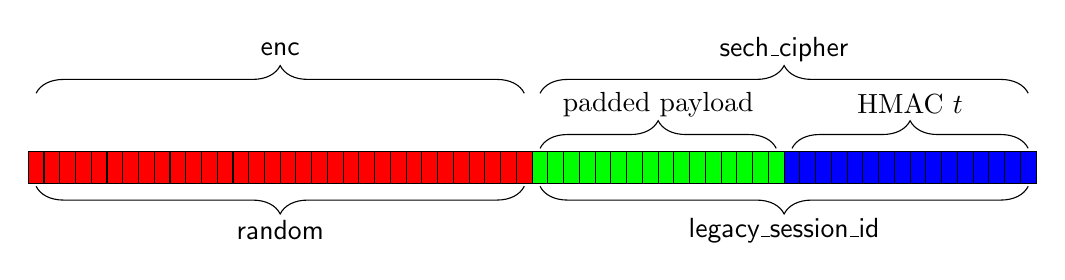
\begin{tikzpicture}

    \def\enclen{\sechfiveenclen}
    \def\taglen{\sechfivetaglen}
    \def\servernamelen{\sechfiveservernamelen}
    \def\randomlen{\sechfiverandomlen}

% Define the box width
\def\boxwidth{0.2}
\def\shiftclose{0.1}
\def\shiftfar{0.8}
\def\textshift{0.7}



% Define colors
\colorlet{color1}{red}
\colorlet{color2}{green}
\colorlet{color3}{blue}
\colorlet{color4}{purple}

    \pgfmathsetmacro{\encbegin}{0}
    \pgfmathsetmacro{\encend}{\encbegin+\enclen-1}
    \pgfmathsetmacro{\ciphertextbegin}{\encend+1}
    \pgfmathsetmacro{\ciphertextend}{\ciphertextbegin+\servernamelen+\randomlen-1}
    \pgfmathsetmacro{\tagbegin}{\ciphertextend+1}
    \pgfmathsetmacro{\tagend}{\tagbegin+\taglen-1}

    \pgfmathsetmacro{\servernamebegin}{\encend+1}
    \pgfmathsetmacro{\servernameend}{\servernamebegin+\servernamelen-1}
    \pgfmathsetmacro{\randombegin}{\servernameend+1}
    \pgfmathsetmacro{\randomend}{\randombegin+\randomlen-1}

% Draw the 64 boxes using the box width and color them based on \i
\foreach \i in {0, 1, ..., 63} {
    \ifnum\i<\ciphertextbegin
        \colorlet{currentcolor}{color1}
    \else\ifnum\i<\tagbegin
        \colorlet{currentcolor}{color2}
    \else
        \colorlet{currentcolor}{color3}
    \fi\fi
    \node[draw, fill=currentcolor, minimum width=\boxwidth cm, minimum height=2*\boxwidth cm, inner sep=0pt, outer sep=0pt] at (\i*\boxwidth, 0) {};
}

% Draw braces at the bottom
\draw[decorate,decoration={brace,amplitude=10pt,mirror,raise=4pt},yshift=-\shiftclose cm]
    (0,0) -- (31*\boxwidth,0) node[midway,yshift=-\textshift cm]{\var{random}};

\draw[decorate,decoration={brace,amplitude=10pt,mirror,raise=4pt},yshift=-\shiftclose cm]
    (32*\boxwidth,0) -- (63*\boxwidth,0) node[midway,yshift=-\textshift cm]{\var{legacy\_session\_id}};

% Draw braces at the top
\draw[decorate,decoration={brace,amplitude=10pt,raise=4pt},yshift=\shiftfar cm]
    (\encbegin,0) -- (\encend*\boxwidth,0) node[midway,yshift=\textshift cm]{\var{enc}};

% Draw braces at the top
\draw[decorate,decoration={brace,amplitude=10pt,raise=4pt},yshift=\shiftfar cm]
    (\servernamebegin*\boxwidth,0) -- (63*\boxwidth,0) node[midway,yshift=\textshift cm]{\var{sech\_cipher}};

\draw[decorate,decoration={brace,amplitude=10pt,raise=4pt},yshift=\shiftclose cm]
(\tagbegin*\boxwidth,0) -- (\tagend*\boxwidth,0) node[midway,yshift=\textshift cm]{HMAC $t$};

\draw[decorate,decoration={brace,amplitude=10pt,raise=4pt},yshift=\shiftclose cm]
(\ciphertextbegin*\boxwidth,0) -- (\ciphertextend*\boxwidth,0) node[midway,yshift=\textshift cm]{padded payload};

% \draw[decorate,decoration={brace,amplitude=10pt,raise=4pt},yshift=\shiftclose cm]
(\servernamebegin*\boxwidth,0) -- (\servernameend*\boxwidth,0) node[midway,yshift=\textshift cm]{servername};

% \draw[decorate,decoration={brace,amplitude=10pt,raise=4pt},yshift=\shiftclose cm]
% (\randombegin*\boxwidth,0) -- (\randomend*\boxwidth,0) node[midway,yshift=\textshift cm]{nonce};

\end{tikzpicture}
\end{document}

